\subsection{Simulation}

\begin{frame}{Simulation}{LOS Coverage Map}
  \begin{block}{Parameters taken into account for map simulation:}

	  \begin{itemize}
	  	\item Terrain elevation
	  	\item Curvature of the Earth
	  	\item Altitude of UA and GS
	  \end{itemize}

	  \begin{figure}
        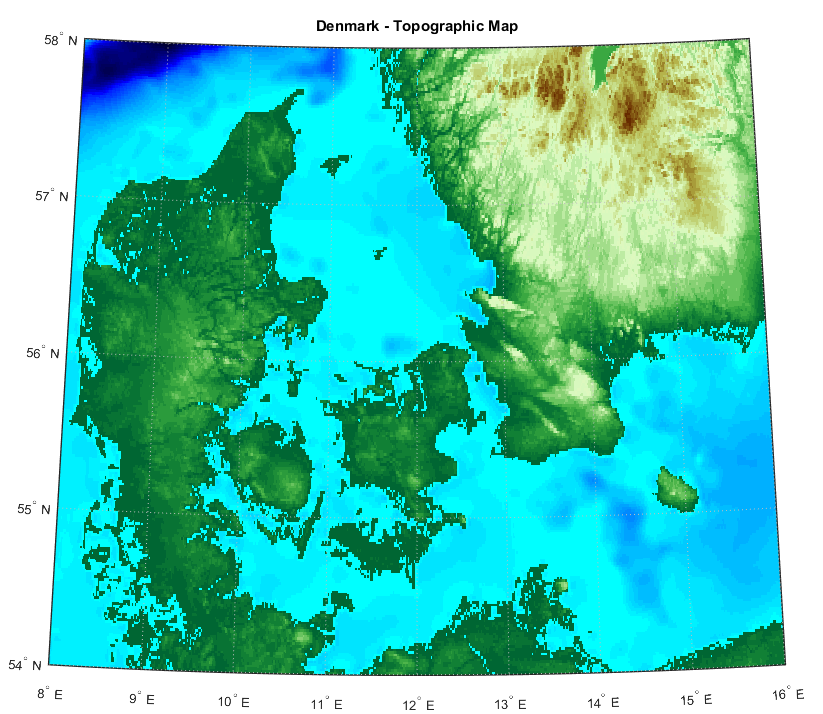
\includegraphics[scale=0.26]{../report/figures/dk_map.png}
      \end{figure}
  
  \end{block}
\end{frame}

\begin{frame}{Simulation}{LOS Coverage Map}
  \begin{block}{Working Principle}
	  \begin{itemize}
	  	\item Import topography map
	  	\item Input GS and UA altitude
	  	\item Choose GS and UA locations on map to plot LOS distance
	  	\item Choose GS location on map to plot LOS coverage map
	  \end{itemize}
  \end{block}
\end{frame}

\begin{frame}{Simulation}{LOS between UA and GS} 
  	\begin{figure}
        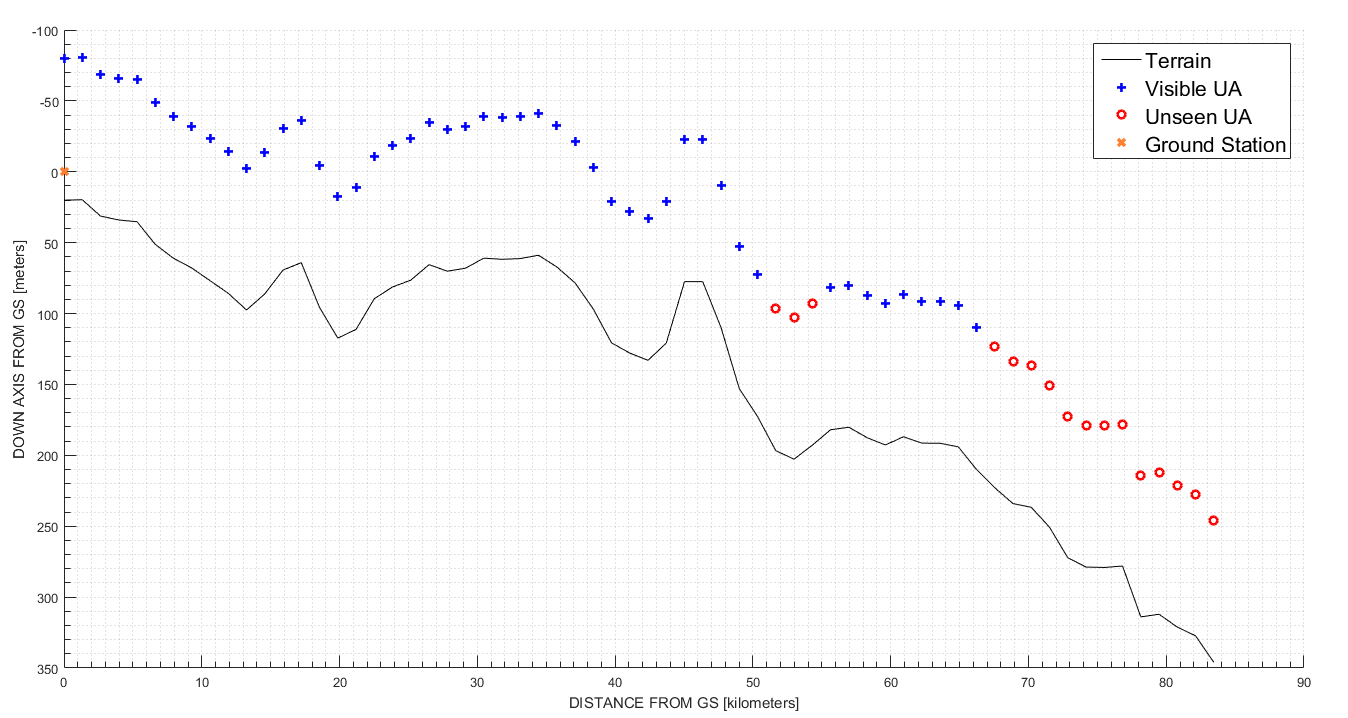
\includegraphics[scale=0.29]{../report/figures/los_2points.png}
    \end{figure}
\end{frame}

\begin{frame}{Simulation}{LOS Coverage Map} 
  	\begin{figure}
        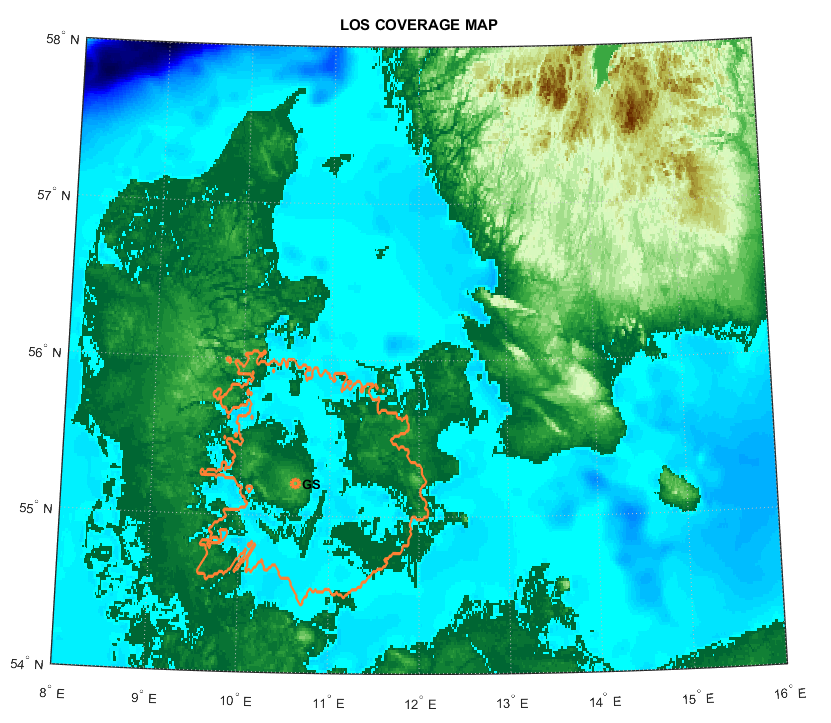
\includegraphics[scale=0.40]{../report/figures/los_odense.png}
    \end{figure}
\end{frame}

\begin{frame}{Simulation}{2D UAS}
	\begin{block}{2D UAS Block Diagram}

		\begin{figure}
	        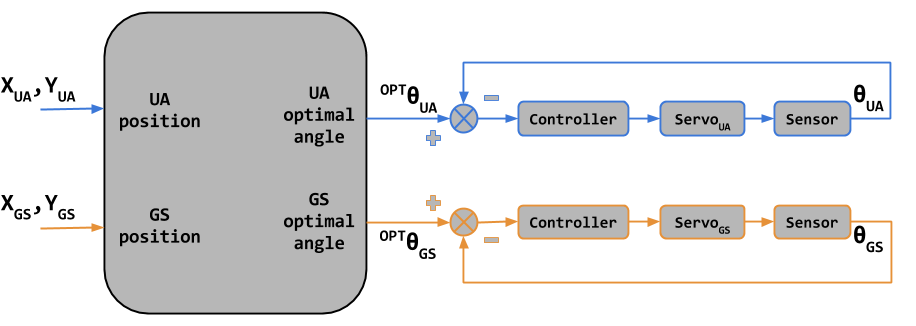
\includegraphics[scale=0.32]{figures/2D_system.png}
	    \end{figure}
    \end{block}
\end{frame}

\begin{frame}{Simulation}{3D UAS}
  \begin{block}{3D UAS Block Diagram}

		\begin{figure}
	        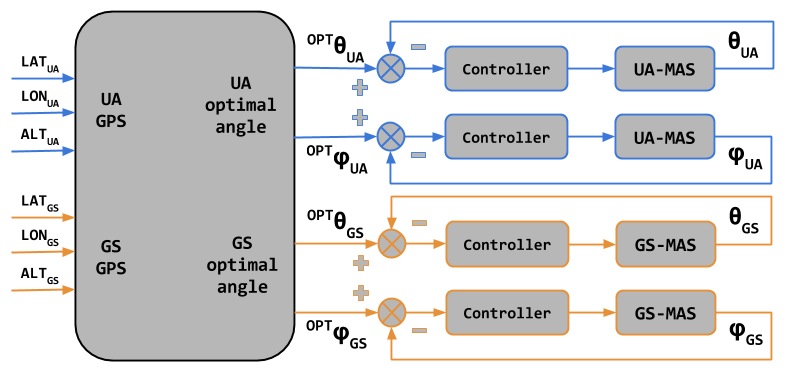
\includegraphics[scale=0.35]{figures/3D_system.png}
	    \end{figure}
  \end{block}
\end{frame}